\documentclass[border=4pt]{standalone}
% shared style for all PyTBA topology diagrams (\input by each standalone file)
\usepackage{mathpazo}
\usepackage{amsmath}
\usepackage{tikz}
\usetikzlibrary{positioning,arrows.meta,calc,decorations.pathreplacing,fit,backgrounds}
\tikzset{
  host/.style={draw=blue!55!black, fill=blue!7, rounded corners=2pt, align=center,
               minimum height=9mm, minimum width=22mm, font=\small},
  blk/.style={draw=black!60, fill=black!4, rounded corners=2pt, align=center,
              minimum height=8mm, font=\small},
  chan/.style={draw=orange!70!black, fill=orange!8, rounded corners=2pt, align=center,
               minimum height=9mm, font=\small},
  lossbox/.style={draw=red!70!black, fill=red!6, rounded corners=2pt, align=center, font=\footnotesize},
  data/.style={-{Stealth[length=2.2mm]}, thick},
  ack/.style={-{Stealth[length=2mm]}, dashed, black!60},
  lbl/.style={font=\footnotesize, align=center},
  brace/.style={decorate, decoration={brace, amplitude=4pt}, thick, black!70},
}

\begin{document}
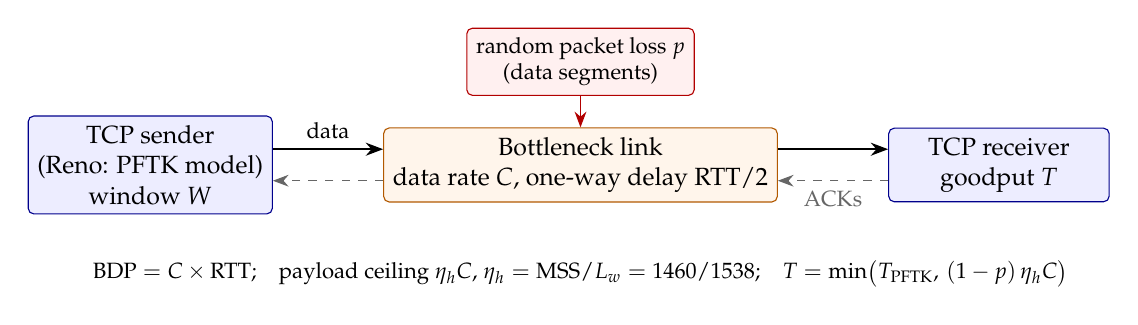
\begin{tikzpicture}
\node[host, minimum width=28mm] (s) {TCP sender\\(Reno: PFTK model)\\window $W$};
\node[chan, right=14mm of s, minimum width=44mm] (l) {Bottleneck link\\data rate $C$, one-way delay RTT/2};
\node[lossbox, above=4mm of l] (p) {random packet loss $p$\\(data segments)};
\node[host, right=14mm of l, minimum width=28mm] (r) {TCP receiver\\goodput $T$};
\draw[data] ($(s.east)+(0,2mm)$) -- node[lbl, above] {data} ($(l.west)+(0,2mm)$);
\draw[data] ($(l.east)+(0,2mm)$) -- ($(r.west)+(0,2mm)$);
\draw[ack] ($(r.west)+(0,-2mm)$) -- node[lbl, below] {ACKs} ($(l.east)+(0,-2mm)$);
\draw[ack] ($(l.west)+(0,-2mm)$) -- ($(s.east)+(0,-2mm)$);
\draw[-{Stealth[length=2mm]}, red!70!black] (p) -- (l);
\node[lbl, below=6mm of l] {$\mathrm{BDP}=C\times\mathrm{RTT}$;\quad payload ceiling $\eta_h C$, $\eta_h=\mathrm{MSS}/L_w=1460/1538$;\quad
  $T=\min\!\big(T_{\mathrm{PFTK}},\,(1-p)\,\eta_h C\big)$};
\end{tikzpicture}
\end{document}
